\documentclass[10pt,letterpaper]{article}
\usepackage[utf8]{inputenc}
\usepackage{amsmath}
\usepackage{amsfonts}
\usepackage{amssymb}
\usepackage{graphicx}
\usepackage{algorithm}
\usepackage{algorithmicx}
\usepackage{algpseudocode}
\usepackage{setspace}



\newcommand{\R}{\mathbb{R}}
\renewcommand{\thesubsection}{\thesection.\alph{subsection}}

\author{Brock Ellefson}
\title{CSCI432 HW4}
\begin{document}

\maketitle

\section{Describe one thing
that you already do well in your academic writing,
and one thing that you will work on improving
throughout the remainder of this class}

When it comes to writing proof, I think I have one major crux. I rush through it. Often times I have the concept correct, and show that I understand the problem being presented, however, I fail to fully express my thoughts and process of approaching the proof. Towards the beginning of the semester, I was getting frustrated whenever I got the proof 'correct' but was getting docked points. I understand now that I was making proofs very very similar to this:
\\
	\begin{figure}[h]
		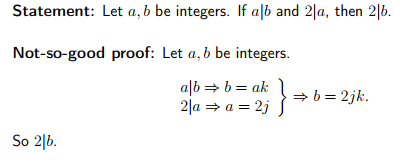
\includegraphics[scale = .75]{badproof.png}
	\end{figure}
\\
I would often forget to write out hypothesis and conclusions, even not defining new variables. After realizing these flaws in my proofs, I've been trying to improve my  formality. Its been a slow process but I believe I'm improving in comparison to the first few proofs we did in class.\\
\\
However, I think a strength I possess in academic writing is my step by step process to proving my proof. For example, in inductive proofs, I often forget my conclusion and problem statement, but I always believed my inductive hypothesis and inductive steps where always pretty solid.

\section{ Prove that the L$_{p}$ distance is a distance metric.}

Prove that the L$_{p}$ distance is a distance metric.\\
L$_{p}$ = d$_{p}$(x,y) = $\Vert$(x$_{1}$ - y$_{1}$)$^{p}$ + (x$_{2}$ - y$_{2}$)$^{p}$ $\Vert$$^{\frac{1}{p}}$ \\
To be a distance metric, you must satisfy 4 requirements:\\
Let X = discrete space\\
A metric is a function d: X x X $\rightarrow$ $\R$ such that:
\begin{enumerate}
  \item d(x,y) = d(y,x)
  \item d(x,y) = 0 $\Leftrightarrow$ x = y
  \item d(x,y) + d(y,z) $\geq$ d(x,z)
  \item d(x,y) $\geq$ 0
\end{enumerate}
So,\\
Given p = 1, then\\
d$_{1}$(x,y) = $\Vert$(x$_{1}$ - y$_{1}$)$^{1}$ + (x$_{2}$ - y$_{2}$)$^{1}$ $\Vert$$^{1}$ \\
= $\Vert$(x$_{1}$ - y$_{1}$)$^{1}$ + (x$_{2}$ - y$_{2}$)$^{1}$$\Vert$\\
= $\delta$\\
\\
d$_{1}$(y,x) = $\Vert$(y$_{1}$ - x$_{1}$)$^{1}$ + (y$_{2}$ - x$_{2}$)$^{1}$ $\Vert$$^{1}$ \\
= $\Vert$(y$_{1}$ - x$_{1}$)$^{1}$ + (y$_{2}$ - x$_{2}$)$^{1}$$\Vert$\\
= $\delta$\\
$\forall$ x,y $\in$ L$_{p}$, d(x,y) = $\delta$ and d(y,x) = $\delta$. $\delta$ = $\delta$. This satisfies condition 1.\\

$\forall$ x,y $\in$ L$_{p}$, if  d(x,y) = 0 then x and y are located at the same coordinates. Therefore x = y. This satisfies condition 2.


\section{Recall the randomized
quicksort algorithm}

\subsection{Give pseudocode for a version of this algorithm
that does not use recursion}


\begin{algorithm}\caption{\textsc{Quicksort}}\label{alg:Quicksort}
 \begin{algorithmic}[1]
 \State \textbf{Procedure} Sort( \texttt{A})
\State \texttt{maxdepth} = $2\lfloor \textit{log} \| \texttt{A} \|  \rfloor $
 \State Introsort( \texttt{A}, \texttt{maxdepth})
 \State ~
 \State \textbf{Procedure} Introsort( \texttt{A}, \texttt{maxdepth})
   \State {\bf in:} \texttt{A}, \texttt{maxdepth}
   

\State {$n \leftarrow |\texttt{A}|$}
\State ~

\If{$n \leq 1$}
	\State {\textbf{return}}
\ElsIf{\texttt{maxdepth} = 0}
	\State \textsc{heapsort}(\texttt{A})
\Else
	\State $p \leftarrow$ \textsc{partition}(\texttt{A})
    \State \textsc{introsort}(\texttt{A}[0:$p$],\ \texttt{maxdepth - 1})
    \State \textsc{introsort}(\texttt{A}[$p + 1$:$n$],\ \texttt{maxdepth} $- 1$)
    
\EndIf

 \end{algorithmic}
\end{algorithm}

\end{document}


